\section{Problem No.3}
\subsection{Problem Description:}
\[
u_{t} = u_{xx},\;\; 0<x<1\\
u(0,t) =1,\;\; u(1,t)=0\\
u(x,0)=\begin{cases}
         1\;\;\; if \;\;x<0.5\\
         0\;\;\; if\;\; x\geq 0.5
         \end{cases}
\]


\begin{enumerate}
\item Use Crank-Nicolson with grid spacing $\Delta x=0.02$ and time step 0.1 to solve the problem up to time $t=1$. Comment on your results. What is wrong with the solution?
\item Give a mathematical argument to explain the unphysical behavior you observed in the numerical solution.
\item Repeat the simulation using BDF2, and discuss why the unphysical behavior is not present in the numerical solution for any time step. 
\end{enumerate}
\subsection{Solution:}
\paragraph{Crank-Nicolson:}
Following the same procedure described in Section \ref{prob2_sol}, we can derive a similar set of linear equations for Crank-Nicolson. The difference lies withing the values of the coefficients $A,B,C,$ and $D$ as follows:
$$ A = 1+\Delta t \frac{1}{(\Delta x)^{2}},\\
B=C=- \frac{\Delta t}{2}\frac{1}{(\Delta x)^{2}},\\
D_{i}^{n} = (1-\Delta t \frac{1}{(\Delta x)^{2}})u_{i}^{n} + \frac{\Delta t}{2}\frac{1}{(\Delta x)^{2}}(u_{i+1}^{n} +u_{i-1}^{n})$$
Thus, the system can be solved using the same LU-Decomposition technique. 

Using $\Delta x =0.02$ and  $\Delta t = 0.1$, the solution is shown in Figure \ref{fig:cn}(a). It is clear that the solution exhibits some nonphysical behavior. It is expected that the initial condition and its discontinuity to wash out at the end. But at $x=0.4$ the solution's discontinuity still persists. Additionally, the amplitude of the exact solution (from the lecture notes) is $|u|=e^{-D\zeta^{2}t}$, where $D=1$. This indicates that if the initial conditions are discontinuities i.e., high spatial frequency (quick change in the function within small distance), it will instantly smoothed out which is not the case here. 

We notice that the unphysical behavior of the solution diminishes if we increase the total time. When the total time is increased up to 10 and 50 (Figure \ref{fig:cn}(b) and (c)), the high frequency components starts to decay. Since Crank-Nicolson scheme is stable, then it is possible that the nonphysical behavior is due to the rate of decay of the high frequency components specially that we have large discontinuity in the initial conditions. This shall be investigated next. 

 \begin{figure}[!tbh]
 \centering 
  \subfloat [time = 1]{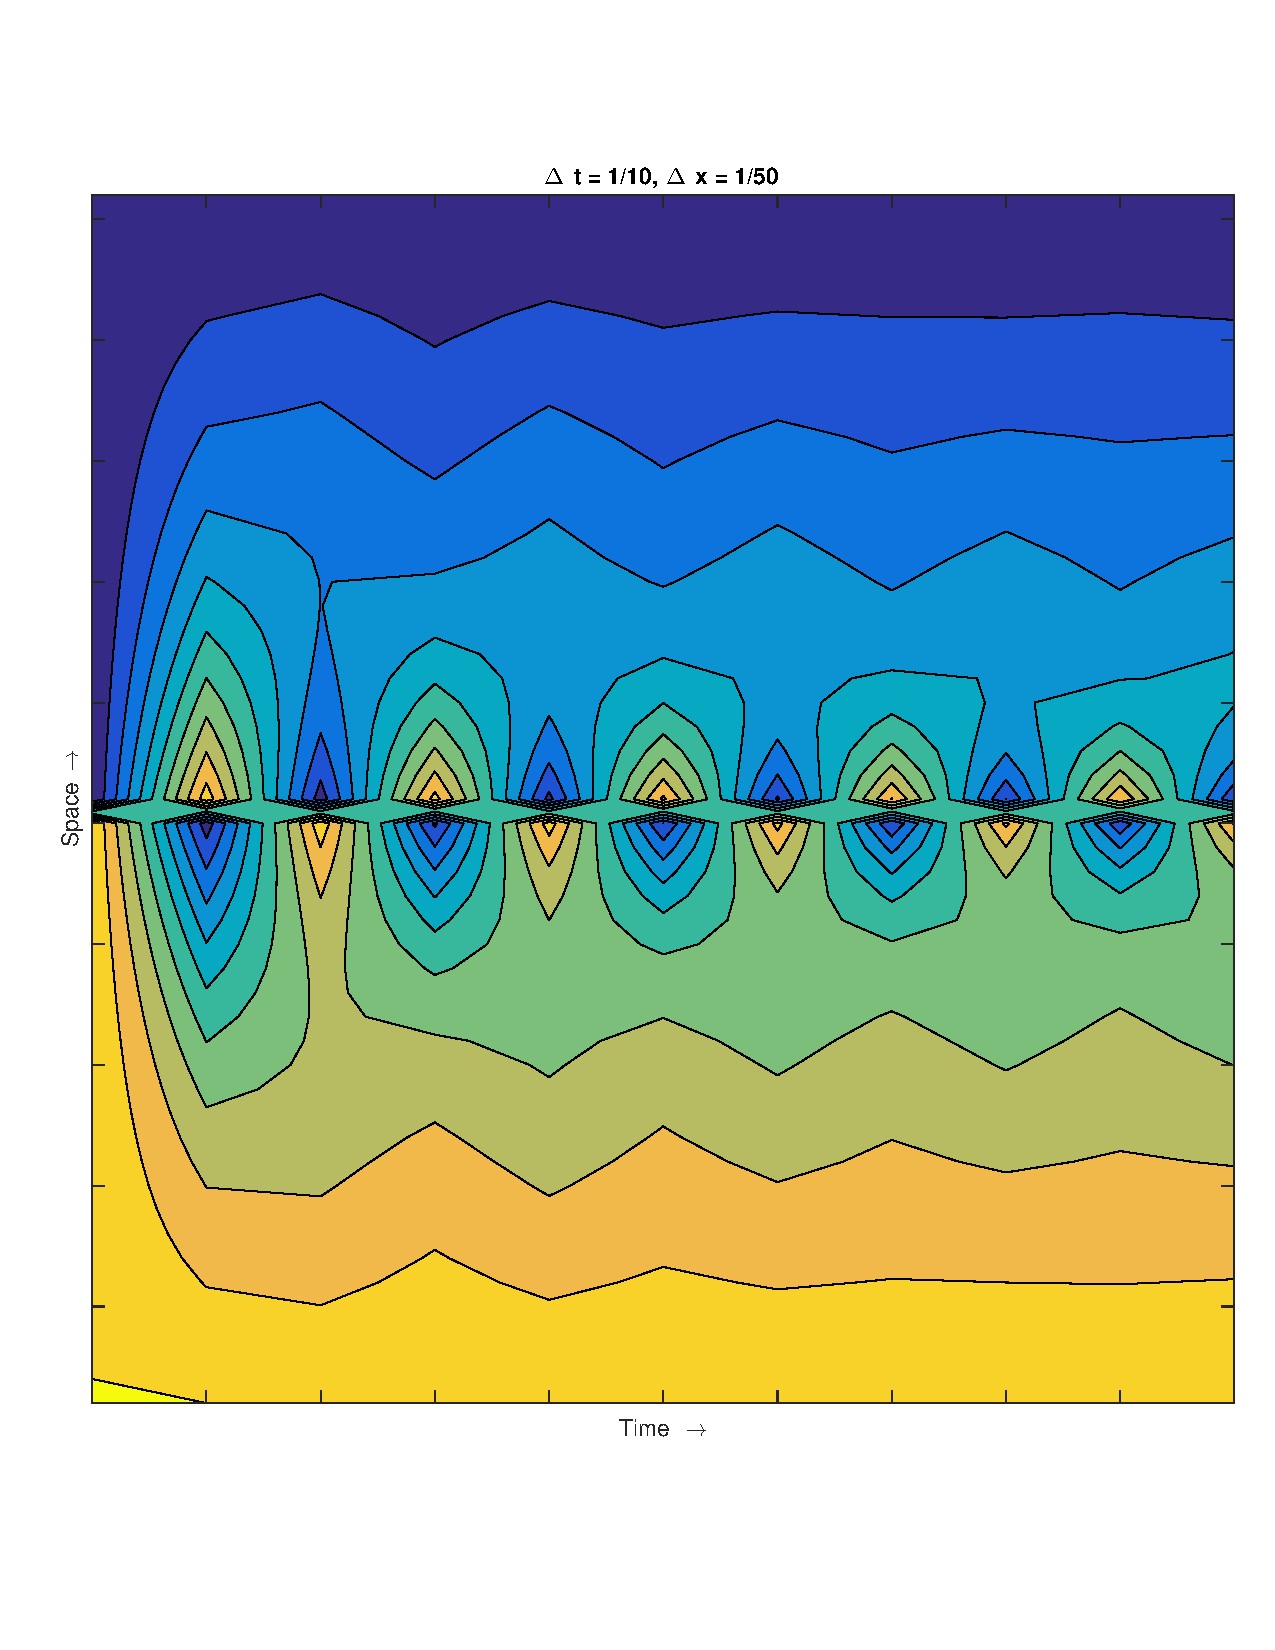
\includegraphics[scale=0.3]{fig/X10_T50_time1.pdf}}  
  \subfloat [time = 10]{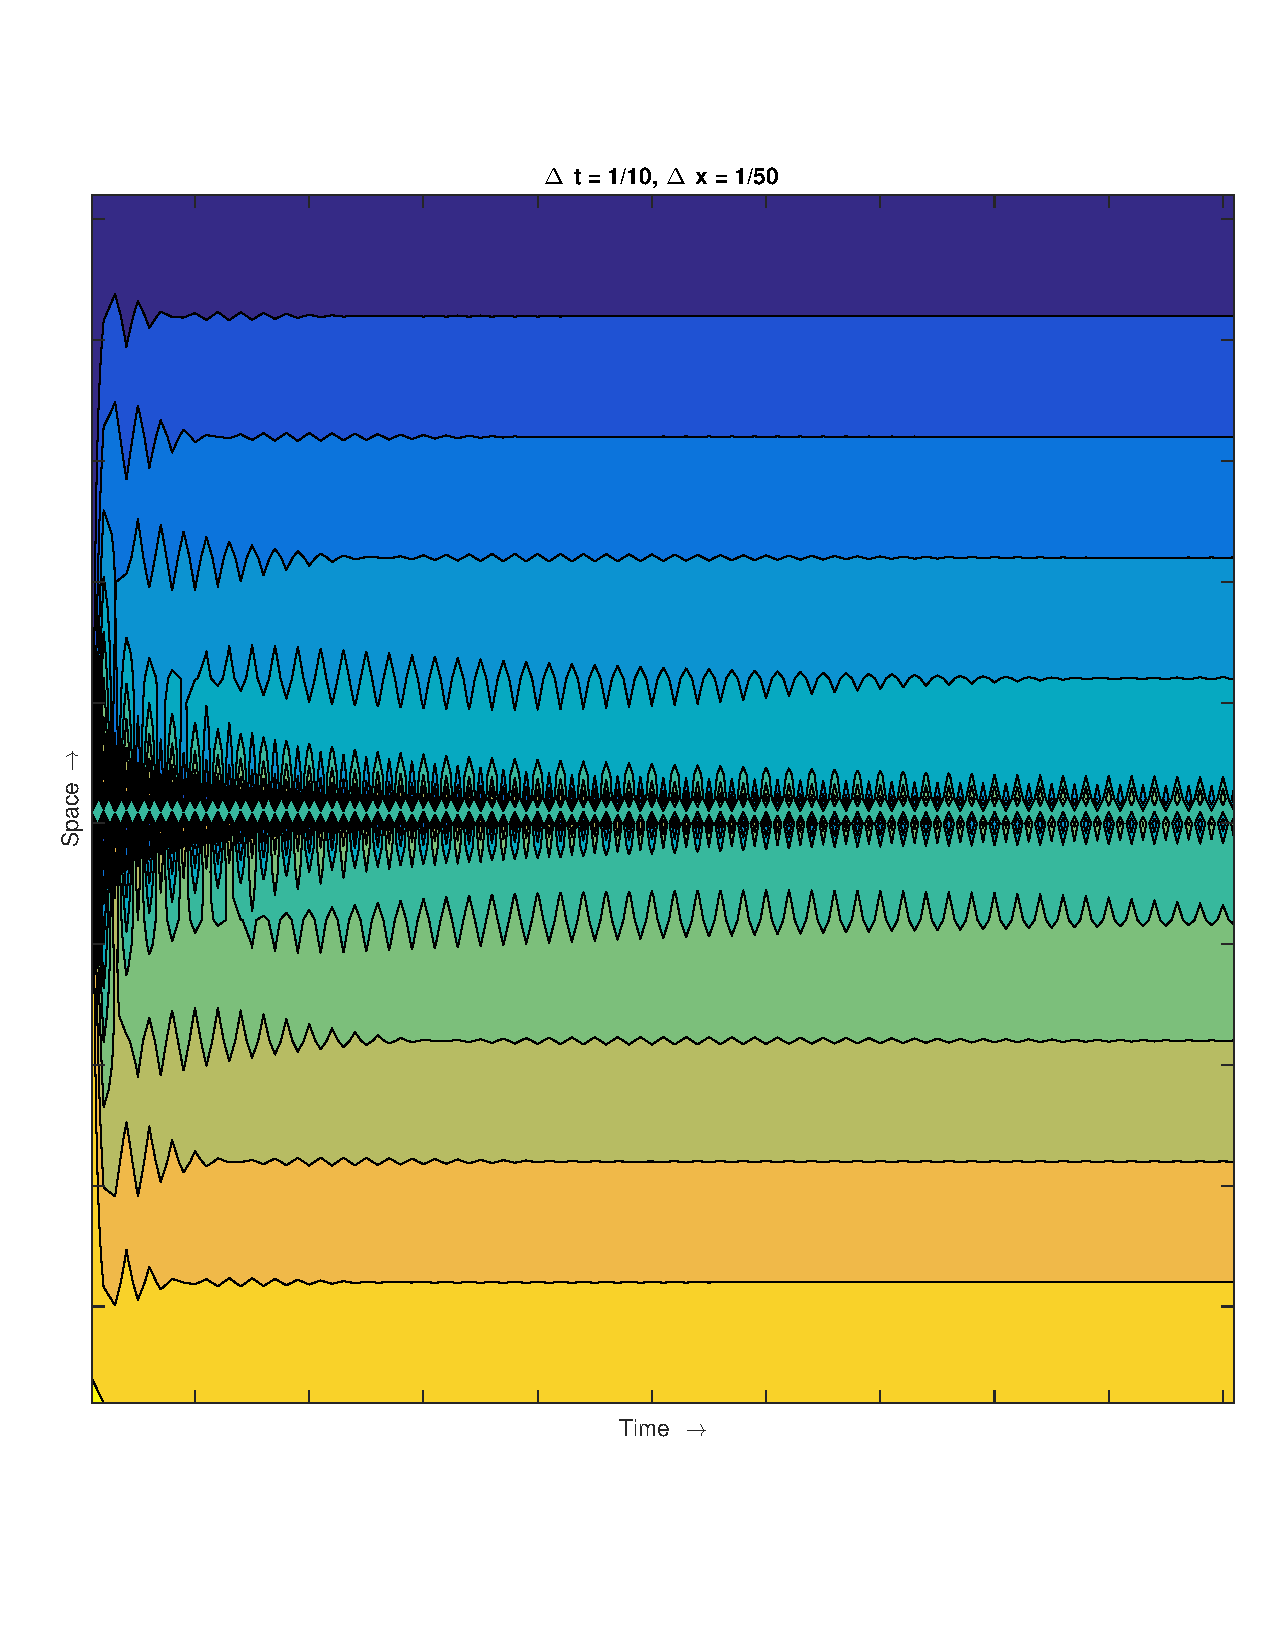
\includegraphics[scale=0.3]{fig/X10_T50_time10.pdf}}  
  \subfloat [time = 50]{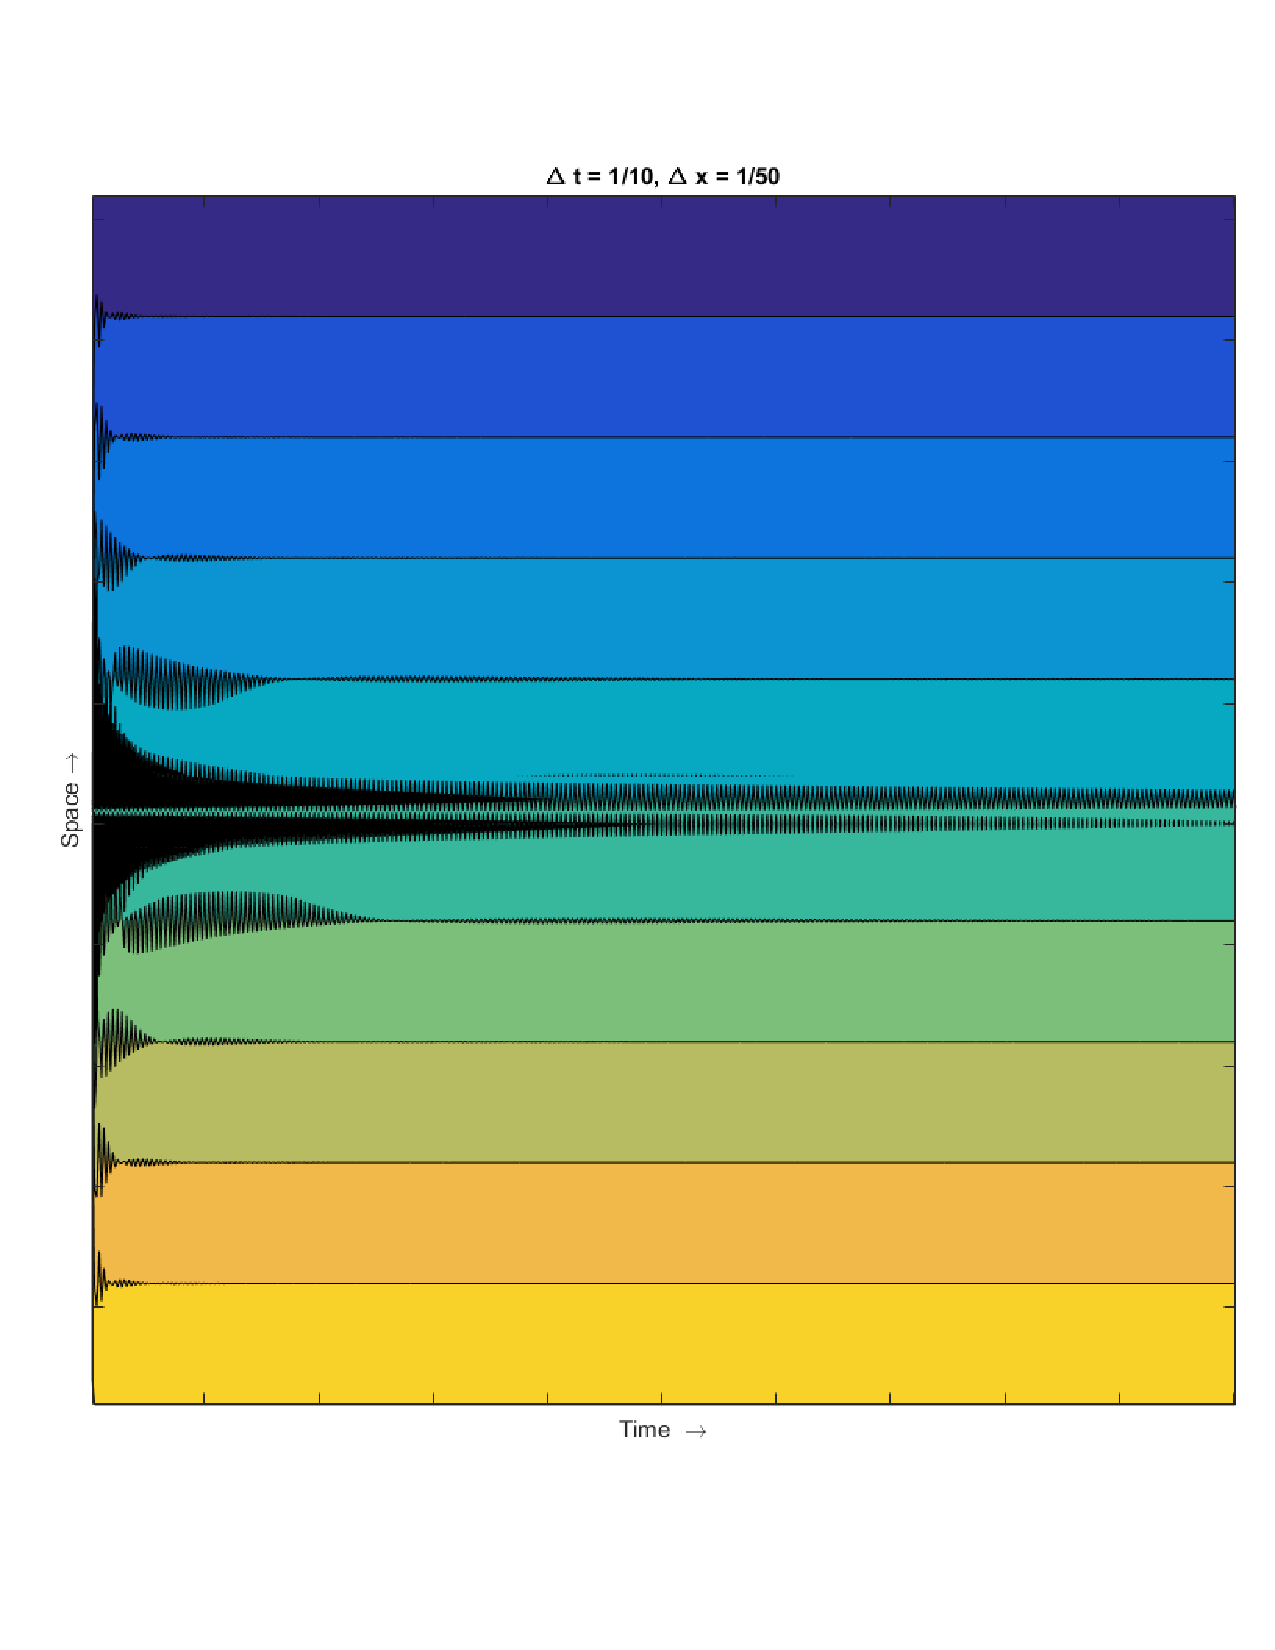
\includegraphics[scale=0.3]{fig/X10_T50_time50.pdf}}  
  \caption{Solution of Problem 3 using Crank-Nicolson scheme with $\Delta x=0.02$ and $\Delta t=0.1$ up to time t=1 (a), t=10 (b) and t=50 (c).}
   \label{fig:cn}
\end{figure} 
\paragraph{Mathematical argument for the nonphysical behavior:}
We would like here to investigate the \emph{amplification factor} of diffusion equation above under Crank-Nicolson scheme. The amplification factor relates the solution of two successive time steps in the Fourier space such that $\hat{u}^{n+1}=g(\zeta)\hat{u}^n$, where $g(\zeta)$ is the amplification factor for the method at wave number $\zeta$\cite{leveque2007finite}. Thus, the amplification factor gives a good indication to what happens to the different frequencies components as we march in time. Notice that for Crank-Nicolson, $|g(\zeta)|\leq 1$ and thus the scheme is A-stable. But if $|g(\zeta)| \approx 1$, then the solution from one time step to another does not change much and the high frequencies persists which looks like the case here. 

Following the derivation of the amplification factor for the diffusion equation under the Crank-Nicolson scheme in \cite {leveque2007finite} (equations 9.27 and 9.28), 
$$g(\zeta) = \frac{1+\frac{\Delta t}{\Delta x^{2}}(cos(\Delta x\zeta)-1)}{1-\frac{\Delta t}{\Delta x^{2}}(cos(\Delta x\zeta)-1)}$$ 
The high frequencies occur at $cos(\Delta x\zeta)\approx\pi$, and the amplification factor becomes
$$g(\zeta) = \frac{1-2\frac{\Delta t}{\Delta x^{2}}}{1+2\frac{\Delta t}{\Delta x^{2}}}$$ 

For $\Delta x =0.02$ and $\Delta t=0.1$, $|g(\zeta)|=0.995$ which is too close to 1.0 which explains the nonphysical behavior in the solution. This also gives an intuition for how to solve such behavior, either by allowing enough time for the solution to converge and for the high frequncies to wash out as shown in Figure \ref{fig:cn}(c) or choose different time and space steps such that $|g(\zeta)|\leq0.5$.

\paragraph{BDF2:}
Here we try to solve the same problem using BDF2 scheme using the same boundary and initial conditions. The discretized PDE under BDF2 is

$$
\frac{3u_{i}^{n+1}-4u_{i}^{n}+u_{i}^{n-1}}{2\Delta t} = \frac{u_{i+1}^{n+1} -2u_{i}^{n+1}+u_{i-1}^{n+1}}{(\Delta x)^{2}}
$$
After rearrangement, it becomes 
$$
(3+\frac{4\Delta t}{(\Delta x)^{2}})u_{i}^{n+1} - \frac{2\Delta t}{(\Delta x)^2}u_{i+1}^{n+1} - \frac{2\Delta t}{(\Delta x)^2}u_{i-1}^{n+1} = 4u_{i}^{n} - u_{i}^{n-1}
$$

or
$$
Au_{i}^{n+1} + Bu_{i+1}^{n+1} +Cu_{i-1}^{n+1} = D_{i}^{n}
$$
\vspace{0.2mm}

where $A = (3+\frac{4\Delta t}{(\Delta x)^{2}}), \; B=C=- \frac{2\Delta t}{(\Delta x)^2}$ and $D_{i}^{n}=4u_{i}^{n} - u_{i}^{n-1}$

Thus, to solve at certain time step, information from two previous time steps should be available. To solve this issue, we use BDF1 to solve the PDE for the first time step $n=1$. Then we use BDF2 system to solve subsequent time steps.

For BDF1, the discretized PDE is
$$
\frac{u_{i}^{n+1}-u_{i}^{n}}{\Delta t} = \frac{u_{i+1}^{n+1} -2u_{i}^{n+1}+u_{i-1}^{n+1}}{(\Delta x)^{2}}
$$

Which can be written in the form 
$$
Au_{i}^{n+1} + Bu_{i+1}^{n+1} +Cu_{i-1}^{n+1} = D_{i}^{n}
$$


where $A = (1+\frac{2\Delta t}{(\Delta x)^{2}}), \; B=C=- \frac{\Delta t}{(\Delta x)^2}$ and $D_{i}^{n}=u_{i}^{n}$.

The system of equation from BDF1 and BDF2 can be solved using the same LU-Decomposition solver. The result is shown in Figure \ref{fig:bdf2}, where the nonphysical behavior no longer exists. 

 \begin{figure}[!tbh]
 \centering  
  {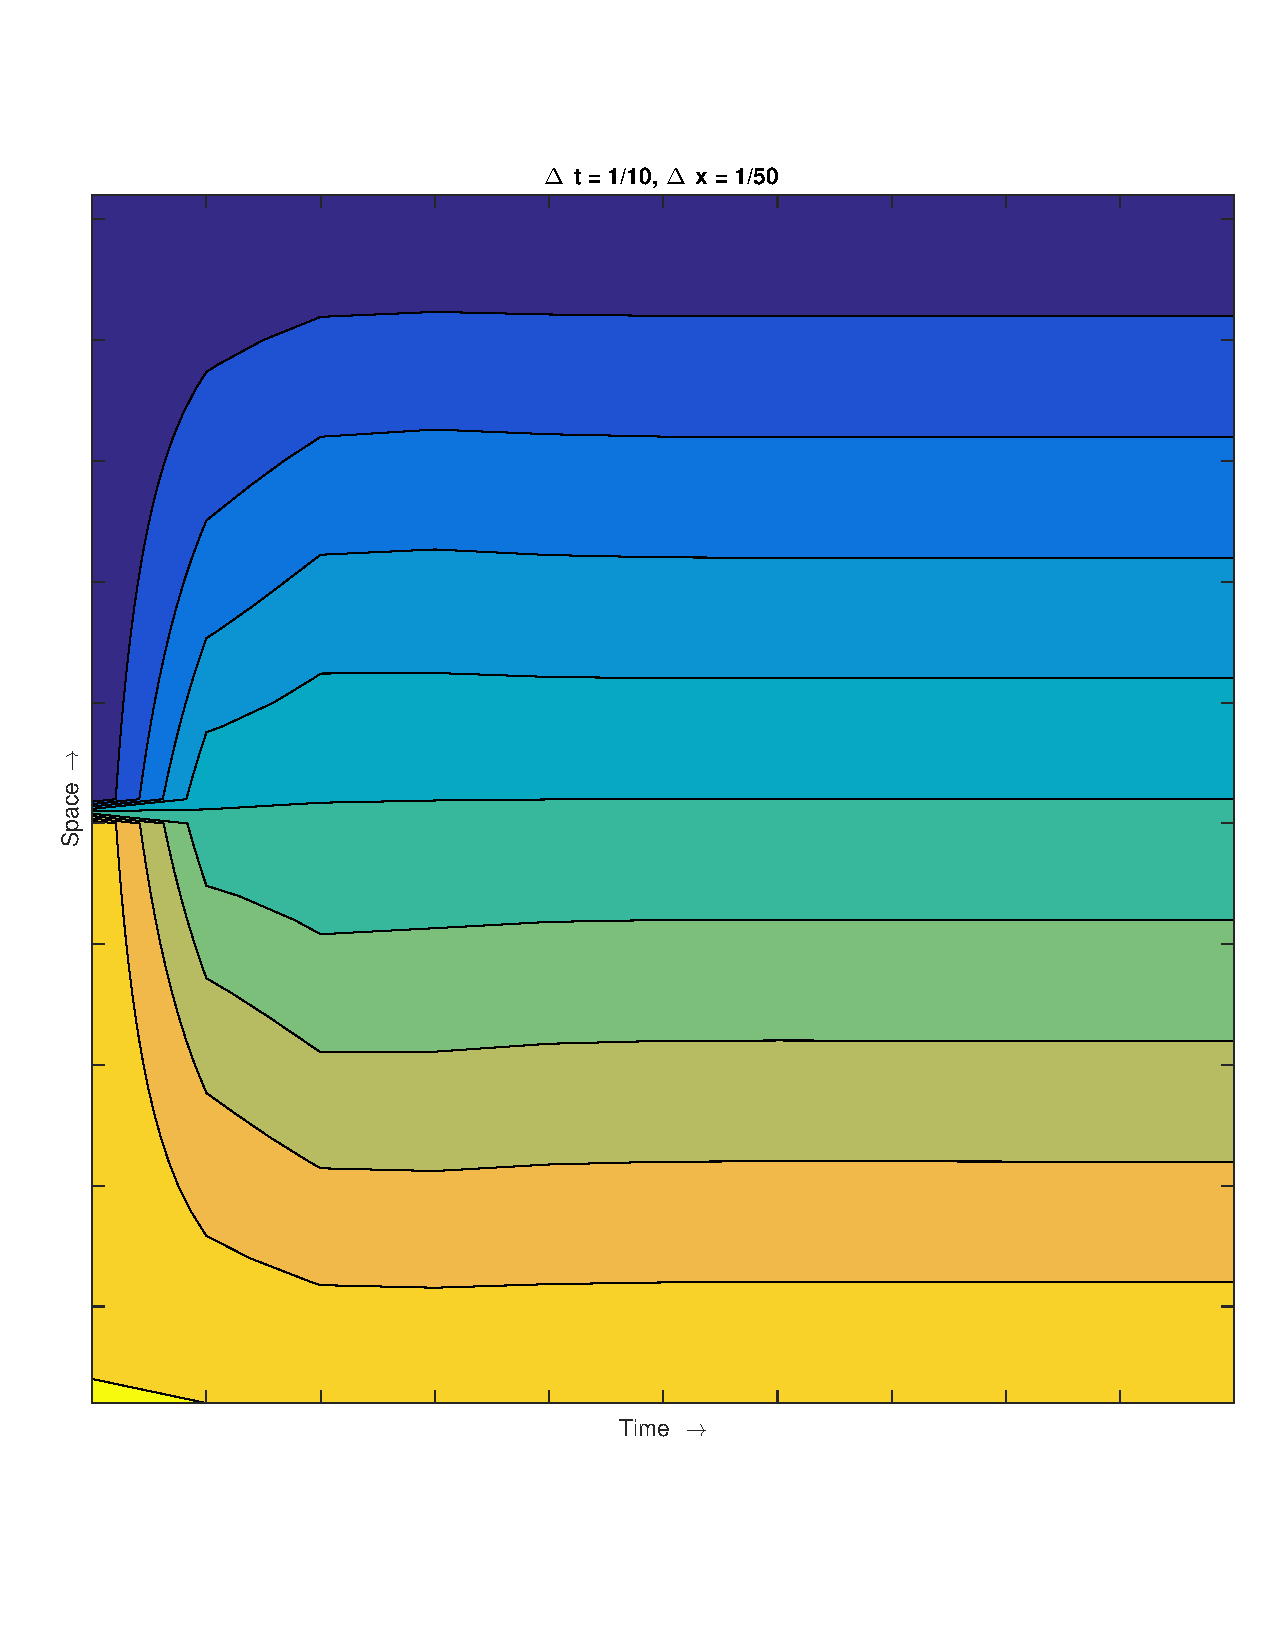
\includegraphics[scale=0.4]{fig/X10_T50_BFD2.pdf}}  
  \caption{Solution of Problem 3 using BDF2 scheme with $\Delta x=0.02$ and $\Delta t=0.1$ up to time t=1, and using BDF1 to solve the first time step.}
   \label{fig:bdf2}
\end{figure} 

\paragraph{BDF2 Amplification Factor:} To explain why the nonphysical behavior no longer exists under BDF2 scheme, we derive the amplification factor for the specified boundary and initial conditions. It is expected that the amplification factor to have a value less than 0.5 since the high frequency components vanish rapidly in the solution (Figure \ref{fig:bdf2}). 
Starting with the form the descretized form of the PDE

$$
(3+4\alpha)u_{i}^{n+1} - 2\alpha u_{i+1}^{n+1} - 2\alpha u_{i-1}^{n+1} = 4u_{i}^{n} - u_{i}^{n-1}
$$

where $\alpha = \frac{\Delta t}{(\Delta x)^{2}}$. The solution is of the form $u_{i}^{n}=e^{ij\Delta x \zeta}$, where $j=\sqrt{-1}$. We expect that $u_{i+1}^{n}=g(\zeta)e^{ij\Delta x \zeta}$, where $g(\zeta)$ is the amplification factor at the wave number $\zeta$. Plugging in these expressions in the descretized form of the PDE gives

$$
(3+4\alpha)g(\zeta)e^{ij\Delta x \zeta} -2\alpha g(\zeta)e^{(i+1)j\Delta x \zeta} - 2\alpha g(\zeta)e^{(i-1)j\Delta x \zeta} = 4e^{ij\Delta x \zeta} - (g(\zeta))^{-1}e^{ij\Delta x \zeta}
$$

dividing by $e^{ij\Delta x \zeta}$

$$
(3+4\alpha)g(\zeta) -2\alpha g(\zeta)e^{j\Delta x \zeta} - 2\alpha g(\zeta)e^{-j\Delta x \zeta} = 4 - (g(\zeta))^{-1}
$$

hence
$$
(g(\zeta))^{2} (3+4\alpha-2\alpha(e^{j\Delta x \zeta} +e^{-j\Delta x \zeta}))-4g(\zeta)+1=0
$$

$$
(g(\zeta))^{2} (3+4\alpha-4\alpha cos(\Delta x \zeta))-4g(\zeta)+1=0
$$

Solving the above equation for $g(\zeta)$ gives

$$
g(\zeta) = \frac{4 \pm \sqrt{16-12-16\alpha +16\alpha cos(\Delta x \zeta)}}{6+8+\alpha-8\alpha cos(\Delta x \zeta)}
$$

As mentioned previously, the high frequency components occurs at $cos(\Delta x \zeta)\approx \pi$. This gives
$$
g(\zeta) = \frac{4 \pm \sqrt{4-32\alpha}}{6+16\alpha}
$$

Substituting with the given initial and boundary conditions values gives $\alpha = 250$. Thus the amplification factor becomes 
$$
g(\zeta) = \frac{4 \pm 89.42j}{4006}
$$

Thus $|g(\zeta)| = 0.02234$, which explains why the high frequency components vanished rapidly in the solution. Additionally, since $g(\zeta)\leq 1$, the scheme is stable.

